\documentclass[11pt]{article}
\usepackage[margin=1in]{geometry}
\usepackage{amsmath,amssymb,amsthm,mathtools}
\usepackage{booktabs,array}
\usepackage{graphicx}
\usepackage{xcolor}
\usepackage[expansion=false]{microtype}
\usepackage[numbers,sort&compress]{natbib}
\usepackage{caption,subcaption}
\usepackage{url}
\usepackage[hidelinks]{hyperref}

% generated by paper/figures.py from data/snapshot.json - do not edit
\newcommand{\snapdate}{2026-10-20}
\newcommand{\usdSn}{USD~0.0019}
\newcommand{\priceSn}{USD~0.05583}
\newcommand{\blockSn}{1.67}
\newcommand{\tempoSn}{2\,156}
\newcommand{\maxringSn}{64}
\newcommand{\simSn}{57.1}
\newcommand{\usdNear}{USD~0.018}
\newcommand{\priceNear}{USD~4.86}
\newcommand{\blockNear}{0.614}
\newcommand{\tempoNear}{5\,864}
\newcommand{\maxringNear}{32}
\newcommand{\simNear}{71.8}
\newcommand{\usdEth}{USD~3.52}
\newcommand{\priceEth}{USD~2438}
\newcommand{\blockEth}{12}
\newcommand{\tempoEth}{300}
\newcommand{\maxringEth}{32}
\newcommand{\simEth}{9.3}
\newcommand{\usdSol}{USD~0.025}
\newcommand{\priceSol}{USD~106}
\newcommand{\blockSol}{0.218}
\newcommand{\tempoSol}{16\,518}
\newcommand{\maxringSol}{32}
\newcommand{\simSol}{124}
\newcommand{\usdSub}{USD~0.0061}
\newcommand{\priceSub}{USD~0.006115}
\newcommand{\blockSub}{6.3}
\newcommand{\tempoSub}{572}
\newcommand{\maxringSub}{64}
\newcommand{\simSub}{15.4}
\newcommand{\subSlope}{5.71}
\newcommand{\subIntercept}{6.4}
\newcommand{\subRtwo}{0.999998}
\newcommand{\subPerBlock}{50}
\newcommand{\subProofSlope}{10.08}
\newcommand{\subProofIntercept}{234}
\newcommand{\nearSlope}{7.51}
\newcommand{\nearIntercept}{6.27}
\newcommand{\nearRtwo}{0.999998}
\newcommand{\ethSlope}{409}
\newcommand{\ethIntercept}{412}
\newcommand{\ethRtwo}{0.999990}
\newcommand{\solSlope}{9.44}
\newcommand{\solIntercept}{2.08}
\newcommand{\solRtwo}{0.999993}
\newcommand{\testsNative}{86}
\newcommand{\testsStarknet}{10}
\newcommand{\testsNear}{32}
\newcommand{\testsEth}{15}
\newcommand{\testsSolana}{13}
\newcommand{\testsPostquant}{3}
\newcommand{\testsSubstrate}{13}
\newcommand{\snSteps}{17\,133}
\newcommand{\snEcop}{19}
\newcommand{\pqRunMs}{8.5}
\newcommand{\pqGas}{44\,740}
\newcommand{\scaleChainSpread}{1\,396}
\newcommand{\scaleMinRatio}{307}
\newcommand{\scaleMaxRatio}{5776}
\newcommand{\scaleM}{256}
\newcommand{\scaleV}{64}
\newcommand{\scalering}{16}
\newcommand{\scalehours}{1}
\newcommand{\scaleK}{24}
\newcommand{\scaleC}{32}
\newcommand{\capDefault}{2.2\times10^{-7}}
\newcommand{\starveDefault}{0.0066}
\newcommand{\capSixteen}{0.0041}
\newcommand{\starveSixteen}{0.061}

% tables are generated; the primitive \input keeps \bottomrule legal after them
\makeatletter\newcommand{\tabinput}[1]{\@@input #1 }\makeatother
% bullets and the \thanks mark from the math fonts: the text versions are
% TS1 glyphs, which pdflatex here only has as bitmaps
\renewcommand{\labelitemi}{$\bullet$}
\makeatletter\def\@fnsymbol#1{\ensuremath{\ifcase#1\or *\or \dagger\or \ddagger\else\fi}}\makeatother

\newtheorem{definition}{Definition}
\newtheorem{theorem}{Theorem}
\newtheorem{proposition}[theorem]{Proposition}
\newtheorem{lemma}[theorem]{Lemma}
\newtheorem{corollary}[theorem]{Corollary}
\theoremstyle{remark}
\newtheorem{remark}{Remark}

\newcommand{\G}{\mathbb{G}}
\newcommand{\Fp}{\mathbb{F}_p}
\newcommand{\Zq}{\mathbb{Z}_q}
\newcommand{\Hp}{H_{\mathrm{p}}}
\newcommand{\Hs}{H}
\newcommand{\negl}{\mathrm{negl}}
\newcommand{\Adv}{\mathsf{Adv}}
\newcommand{\cA}{\mathcal{A}}
\newcommand{\cB}{\mathcal{B}}
\newcommand{\Ring}{\mathcal{R}}
\newcommand{\tg}{\tau}
\newcommand{\str}[1]{\texttt{#1}}

\title{\textbf{ztao: Anonymous Incentive Subnets from Scope-Linkable Ring Signatures, with One Signer and Verifiers on Six Execution Environments}}
\author{The ztao authors\thanks{Source, data and the scripts that generate every number, table and figure in this paper: \texttt{orbit/ztao} (\texttt{paper/collect.py}, \texttt{paper/figures.py}). Measurement snapshot: \snapdate.}}
\date{October 2026}

\begin{document}
\maketitle

\begin{abstract}
In incentive subnets of the Bittensor kind, miners produce work, validators score it, and a consensus rule turns scores into emission. Both roles act under persistent public identities, so a validator can favour or punish a known miner and a miner can identify, and retaliate against, the validator that scored it down. We present \emph{ztao}, a protocol that keeps the rules of such a subnet while removing the identities behind every action. Miners and validators form two public sets of keys. Every action is a scope-linkable ring signature (LSAG) whose key image enforces exactly one action per member per scope. A miner's image in an epoch scope is its pseudonymous \emph{tag}. A validator's image in a per-tag scope is a \emph{nullifier}. A claim re-creates the miner's tag and so can only be made by its owner. We pair this with \emph{Zuma consensus}, a variant of Yuma consensus for validators without identities: every validator weighs one, and each score is clipped to the highest score that half of the validator set supports. We prove that a coalition smaller than half the set cannot raise a tag's consensus above what the honest validators support. One signer produces every signature, and six independently written verifiers check them byte for byte: Cairo on Starknet, Rust/wasm on NEAR, Solidity/Yul on Ethereum, sBPF on Solana, an ink!\ contract on Substrate's pallet-contracts, and an off-chain wasm contract with post-quantum (ML-DSA) receipts. Verification cost is linear in the ring size on every chain we fitted ($R^2 \ge 0.9999$). On Substrate it is $\subIntercept + \subSlope\,n$\,ms of reference time, so a 64-member ring uses 29\% of the per-extrinsic limit. Priced at the mainnet fees and token prices of \snapdate, a ring-4 score costs between \usdSn{} (Starknet, estimated) and \usdEth{} (Ethereum L1); on Astar, a public pallet-contracts chain, it costs \usdSub. Per epoch, the cost grows with miners times validators. We show that the usual compressions, batched weights and multi-epoch claims, link actions that the protocol keeps apart. Secret committees drawn from the validators' own nullifiers, followed by settling each epoch with one validity proof, keep every action unlinkable and are modeled to cut a Bittensor-sized subnet's daily cost by a factor of \scaleMinRatio{} to \scaleMaxRatio{}. Committees cost security, not privacy, and we quantify that cost. We also report what the construction does not give: anonymity is bounded by the ring and by network metadata, it does not survive a quantum adversary, and an earlier ring-selection rule leaked claimants through ring intersection. We describe that leak and the fix we adopted.
\end{abstract}

\section{Introduction}

Bittensor~\cite{bittensor} organises machine-learning work into \emph{subnets}. In each subnet, miners serve a task and validators score the miners; Yuma consensus~\cite{yumadocs} then aggregates the validators' stake-weighted scores into emission. Every participant is a public hotkey, and so every score is attributable. Two problems follow.

\begin{enumerate}
\item \textbf{Favouritism.} A validator that knows which miner it is scoring can favour an affiliated miner or punish a competitor. Its score depends on the miner's identity, not on the work.
\item \textbf{Retaliation and collusion markets.} A miner that knows who scored it down can retaliate or negotiate. A miner and a validator that can recognise each other can contract on scores.
\end{enumerate}

Both problems rely on the parties knowing \emph{who} they are dealing with. Neither needs anything else. Every rule a subnet enforces can be stated without identities: miners are registered; each miner submits once per epoch; each validator scores each submission at most once; payouts follow a consensus rule; and each payout is claimed once, by the miner that earned it. This paper shows that all of these rules can be enforced on chain, by contracts that never learn which member acted.

\paragraph{Approach.} We replace identity with \emph{membership plus a scope-bound pseudonym}. A linkable ring signature~\cite{lww04} proves that ``some member of this public ring signed''. Its key image $I = x\cdot \Hp(\sigma)$ is deterministic in the signer's secret $x$ and a \emph{scope}~$\sigma$. Two signatures by the same key in the same scope therefore share an image, while images in different scopes cannot be linked. Choosing the scopes defines the protocol: (epoch) for miners, (epoch, tag) for validators, and the miner's epoch scope again for claims.

\paragraph{Contributions.}
\begin{itemize}
\item \textbf{Protocol} (Section~\ref{sec:protocol}). Four actions, \emph{submit}, \emph{score}, \emph{settle} and \emph{claim}, built only from scope choices on one LSAG instance over the STARK curve with Poseidon~\cite{poseidon} challenges. We state the security properties the subnet needs and reduce each to a standard property of the signature scheme (Section~\ref{sec:security}).
\item \textbf{Zuma consensus} (Section~\ref{sec:zuma}). A version of Yuma consensus for anonymous validators. We prove a clipping bound for coalitions below the quorum, and show that settling a tag on chain costs at most 101 storage reads.
\item \textbf{One signer, six verifiers} (Section~\ref{sec:impl}). A single Cairo prover and its bit-identical Python port sign for every chain. The verifiers are written natively for Starknet, NEAR, Ethereum, Solana, Substrate and an off-chain post-quantum ledger, and each test suite pins its verifier to signatures made by the Cairo prover. The Substrate verifier is new in this paper (Section~\ref{sec:substrate}).
\item \textbf{Measurements} (Section~\ref{sec:eval}). Linear cost models per chain, fitted from deterministic resource accounting; the per-transaction limit that sets each chain's maximum ring; and mainnet prices per action.
\item \textbf{Cost at scale, privacy kept} (Section~\ref{sec:cost}). A per-epoch cost model whose dominant term grows with miners $\times$ validators, and two ladders of cuts. The common cuts (batched weights, lazy claims) link actions. Secret committees drawn from the nullifiers, followed by private settlement in one validity proof, keep every signature unlinkable and reduce a Bittensor-sized subnet's daily cost \scaleMinRatio--\scaleMaxRatio-fold (modeled).
\item \textbf{Limitations, stated precisely} (Section~\ref{sec:limits}). This includes a ring-intersection leak in our earlier ring-selection rule and its fix.
\end{itemize}

\paragraph{Non-goals.} ztao does not hide \emph{that} someone is a subnet member, how many members there are, or the content of submitted work. It does not provide Sybil resistance~\cite{sybil}, which stays with whoever admits keys to the sets. It does not move tokens: payouts are credits in contract storage, so the system cannot be used as a general-purpose mixer.

\section{Background and related work}\label{sec:related}

\paragraph{Ring signatures and linkability.} Ring signatures~\cite{rst01} let a signer hide among an ad hoc set of public keys. Linkable ring signatures~\cite{lww04} add a tag that reveals when two signatures share a signer. The \emph{key image} of CryptoNote~\cite{cryptonote} and Monero's RingCT~\cite{ringct} is the same idea, used there to prevent double spends. Traceable ring signatures~\cite{fs07} make the tag depend on an application-chosen issue, which is what our \emph{scope} is. Bender, Katz and Morselli~\cite{bkm06} give a hierarchy of anonymity and unforgeability definitions, which we use informally. Empirical work on Monero~\cite{kumar17,moser18} shows how ring anonymity erodes in deployment, through decoy selection, temporal analysis and ring intersection. Our Section~\ref{sec:intersection} is an instance of the last of these.

\paragraph{Nullifiers.} Zerocash~\cite{zerocash} prevents double spending with a nullifier derived from a secret and revealed when spending; it proves membership with a SNARK. Our validator nullifier plays the same role with a ring signature instead of a succinct proof. That trades proof size linear in the ring for a transparent, setup-free scheme whose verifier is a few hundred lines on each chain.

\paragraph{Bittensor and Yuma.} In Yuma consensus~\cite{yumadocs}, each validator's weights are clipped to a stake-weighted $\kappa$-majority consensus, and validators earn dividends through exponentially smoothed bonds. Bonds and dividends both need a validator identity that persists across rounds, which is exactly what ztao removes (Section~\ref{sec:zuma}).

\paragraph{Execution environments.} The Starknet STARK curve and Poseidon are native to Cairo~\cite{cairo,stark}. NEAR~\cite{nightshade}, Substrate's pallet-contracts~\cite{polkadot,ink} and our post-quantum ledger all execute WebAssembly~\cite{wasm}, and Ethereum~\cite{yellowpaper} and Solana~\cite{solana} have their own virtual machines. None of the last five has STARK-curve host functions, so each verifier brings its own field and curve arithmetic. Our implementation techniques are classical: Montgomery multiplication~\cite{montgomery85}, simultaneous (Straus) double-scalar multiplication~\cite{straus64}, and batch inversion~\cite{montgomery87}.

\section{The signature scheme}\label{sec:scheme}

\paragraph{Parameters.} Let $p = 2^{251} + 17\cdot 2^{192} + 1$ and let $\G$ be the STARK curve $E: y^2 = x^3 + x + \beta$ over $\Fp$. $\G$ has prime order $q$ and cofactor~1, with generator $G$. Let $\Hs:\Fp^{*}\to\Fp$ be Poseidon (the Hades permutation with Starknet's parameters) over field-element sequences, with ASCII domain tags $\str{zuma-h2p}$, $\str{zuma-msg}$, $\str{zuma-chal}$, $\str{zuma-key}$, $\str{zuma-mine}$ and $\str{zuma-score}$. Challenges $c\in\Fp$ are used as scalars modulo~$q$. Since $|p-q| < 2^{127}$, reducing a uniform element of $\Fp$ modulo~$q$ is within statistical distance $2^{-124}$ of uniform on $\Zq$.

\paragraph{Hash to curve.} $\Hp(\sigma)$ is defined by try-and-increment~\cite{bls01}. Take the least $k\ge0$ for which $X_k = \Hs(\str{zuma-h2p},\sigma,k)$ is the $x$-coordinate of a point of $E$; then $\Hp(\sigma) = (X_k, \min(y,p-y))$. In the random-oracle model~\cite{bellare93} this is a random point whose discrete logarithm to base $G$ is unknown. A verifier may take $y$ as a \emph{hint}. It then checks $y^2 = X_k^3+X_k+\beta$, checks that $y$ is the smaller root, and checks with Euler's criterion that every $X_j$, $j<k$, is a non-residue. A wrong hint therefore never changes the result; it only forfeits the cheaper path.

\paragraph{Keys and canonical rings.} A secret is $x\in\Zq^{*}$, its public key is $P = xG$, and its key identifier is $\mathrm{id}(P) = \Hs(\str{zuma-key},P_x,P_y)$. A ring $\Ring = (P_0,\ldots,P_{n-1})$ is \emph{canonical} if its identifiers are strictly increasing. A verifier rejects every non-canonical ring, so the same key cannot appear twice to make a ring look larger than it is.

\paragraph{Signing.} To sign $m\in\Fp$ in scope $\sigma$ with secret $x$ at position $\pi$ of a canonical ring $\Ring$, the signer computes $I = x\,\Hp(\sigma)$ and
\[ d = \Hs(\str{zuma-msg}, \sigma, m, I, n, P_0,\ldots,P_{n-1}). \]
It picks $\alpha \gets \Zq$ and sets $c_{\pi+1} = \Hs(\str{zuma-chal}, d, \alpha G, \alpha\Hp(\sigma))$. For $i = \pi+1,\ldots,\pi-1$ (indices modulo $n$) it picks $s_i\gets\Zq$ and sets
\[ L_i = s_iG + c_iP_i,\quad R_i = s_i\Hp(\sigma) + c_iI,\quad c_{i+1} = \Hs(\str{zuma-chal}, d, L_i, R_i), \]
and it closes the ring with $s_\pi = \alpha - c_\pi x \bmod q$. The signature is $(c_0, s_0,\ldots,s_{n-1}, I)$.

\paragraph{Verification.} The verifier checks that $\Ring$ is canonical and that every $P_i$ and $I$ lie on $E$. It recomputes $d$, and then $L_i$, $R_i$ and $c_{i+1}$ for $i=0,\ldots,n-1$ starting from $c_0$. It accepts if and only if $c_n = c_0$.

This is the scheme of Liu, Wei and Wong~\cite{lww04} with the group generator for key images replaced by the per-scope point $\Hp(\sigma)$, as in traceable ring signatures~\cite{fs07}. The message digest binds the scope, the message, the image, the ring size and the ring itself. We claim no new cryptography; what the following sections examine is the composition.

\subsection{Properties of the scheme}\label{sec:props}

We use the following properties. All are in the random-oracle model, with $\Hs$ and $\Hp$ as independent random oracles.

\begin{definition}[Unforgeability with respect to insider corruption]
No PPT adversary that may corrupt some ring members and obtain signatures from the others can output a valid signature on a fresh $(\Ring,\sigma,m)$ in which no member of $\Ring$ is corrupted, except with negligible probability.
\end{definition}

\begin{definition}[Scope linkability]
For any scope $\sigma$ and any PPT adversary holding the secrets of $k$ members of the universe of keys, the adversary cannot output $k+1$ valid signatures in scope $\sigma$ with pairwise distinct key images, over rings drawn from that universe, except with negligible probability.
\end{definition}

\begin{definition}[Non-frameability]
No PPT adversary can output a valid signature in scope $\sigma$ whose key image equals $x\,\Hp(\sigma)$ for the secret $x$ of an uncorrupted member, except with negligible probability, even after seeing signatures by that member in other scopes and in $\sigma$ itself.
\end{definition}

\begin{definition}[Anonymity in a fresh scope]
Let $P_0, P_1$ be honest keys in a ring $\Ring$. Suppose the adversary knows the secrets of every other member of $\Ring$ and may obtain signatures by $P_0$ and $P_1$ in any scope other than a challenge scope $\sigma^*$. The adversary is then given a signature in $\sigma^*$ by $P_b$, for a uniform bit $b$. It must not guess $b$ with advantage better than negligible.
\end{definition}

\begin{theorem}\label{thm:scheme}
In the random-oracle model, the scheme is unforgeable with respect to insider corruption, scope linkable and non-frameable if the discrete-logarithm problem is hard in $\G$. It is anonymous in a fresh scope if the decisional Diffie--Hellman (DDH) problem is hard in $\G$.
\end{theorem}

\begin{proof}[Proof sketch]
The proofs follow Liu, Wei and Wong~\cite{lww04}; we note where scopes change them. \emph{Unforgeability and linkability.} By the forking lemma~\cite{ps00}, an adversary that closes a ring can be rewound on the oracle query that fixes some $c_{j+1}$. Two accepting transcripts with $c_j\neq c'_j$ but equal $(L_j,R_j)$ yield $x_j = (s_j - s'_j)/(c'_j - c_j)$ with $P_j = x_jG$ \emph{and} $I = x_j\Hp(\sigma)$. That is, every accepting signature is bound to one ring member's secret, and that secret is consistent with its image. A forgery for an uncorrupted ring therefore yields a discrete logarithm. For linkability, $k+1$ distinct images in one scope with only $k$ known secrets force some extracted $x_j$ to belong to an uncorrupted key, or to be a second logarithm of a corrupted key, which is impossible. \emph{Non-frameability.} An image $x\Hp(\sigma)$ of an honest key, attached to an accepting signature, extracts to $x$, and finding $x$ is discrete logarithm. The honest key's own signatures in $\sigma$ are simulated by programming $\Hs$ (honest-verifier zero knowledge of the underlying $1$-of-$n$ sigma protocol under Fiat--Shamir~\cite{fiatshamir}). \emph{Anonymity.} Given a DDH tuple $(G, X = xG, Y, Z)$, program $\Hp(\sigma^*) = Y$, use $X$ as $P_b$'s key and $Z$ as the challenge image, and simulate the ring by programming $\Hs$. If $Z = xY$ the view is a real signature by $P_b$. Otherwise the image is independent of both keys and $b$ is information-theoretically hidden. Signatures in other scopes are simulated with independent $\Hp$ points of known logarithm $\Hp(\sigma)=r_\sigma G$, using $I_\sigma = r_\sigma X$.
\end{proof}

\begin{corollary}[Cross-scope unlinkability]\label{cor:unlink}
Under DDH in the random-oracle model, the images of one key in distinct scopes $\sigma\neq\sigma'$ are jointly indistinguishable from the images of two independent keys.
\end{corollary}

\section{The protocol}\label{sec:protocol}

A subnet deployment has a \emph{subnet element} $\mathfrak{s}\in\Fp$ that binds every scope to that one contract (Section~\ref{sec:impl} gives its definition per chain), an epoch length \emph{tempo} in blocks, a minimum ring size $n_{\min}$ enforced on chain, and an emission $E$ per epoch. The epoch of a block $b$ is $e = \lfloor b / \mathit{tempo}\rfloor$. The contract keeps two append-only registries, $\mathcal{M}$ (miners) and $\mathcal{V}$ (validators). A key belongs to at most one of them.

\begin{table}[t]
\centering\small
\begin{tabular}{@{}lllll@{}}
\toprule
action & signer & scope $\sigma$ & message & key image \\
\midrule
submit & a miner & $\Hs(\str{zuma-mine},\mathfrak{s},e)$ & work commitment $w$ & the miner's tag $\tg$ \\
score & a validator & $\Hs(\str{zuma-score},\mathfrak{s},e,\tg)$ & score $s\in\{0..100\}$ & a nullifier $\nu$ \\
settle & anyone & -- & $(e,\tg)$ & -- \\
claim & a miner & $\Hs(\str{zuma-mine},\mathfrak{s},e)$ & recipient $r$ & $\tg$ again \\
\bottomrule
\end{tabular}
\caption{The four actions. Here $\tg$ and $\nu$ denote the identifier $\mathrm{id}(I)$ of the key image. The contract checks the ring against the role's registry (\emph{submit}, \emph{claim}: $\mathcal{M}$; \emph{score}: $\mathcal{V}$), checks $n_{\min}\le n\le n_{\max}$, and rejects a repeated image in the same scope.}
\label{tab:actions}
\end{table}

\paragraph{Actions.} \emph{Submit} (by a miner, while epoch $e$ is open) records the miner's tag $\tg$ with commitment $w$; a second submission with the same image is rejected. The epoch's first submit takes a snapshot $V_e = |\mathcal{V}|$. \emph{Score} (by a validator, while $e$ is open, on a tag of $e$) adds $s$ to the tag's histogram $h_\tg[s]$ and spends $\nu$; a second score with the same $\nu$ is rejected. \emph{Settle} (by anyone, after $e$ closes, once per tag) runs Zuma consensus (Section~\ref{sec:zuma}) and stores $(C_\tg, R_\tg)$. \emph{Claim} (by a miner, after every tag of $e$ is settled) verifies a signature in the miner's epoch scope on the recipient $r$, requires its image to be a tag of $e$ that has not been claimed, and credits $\lfloor E\cdot R_\tg/\sum_{\tg'} R_{\tg'}\rfloor$ to $r$.

\paragraph{Relaying.} A transaction's sender is public on every chain we target, so the anonymous actions never check the caller. A member hands its signed payload to any relayer, which posts it and pays the fee. Only registry administration (\emph{register}, \emph{set\_open}) is restricted to the owner.

\subsection{Security of the protocol}\label{sec:security}

\begin{proposition}\label{prop:protocol}
Assume the scheme satisfies Theorem~\ref{thm:scheme}. Then, except with negligible probability, the following hold.
\begin{enumerate}
\item[(P1)] Each miner has at most one tag per epoch, and only registered miners have tags.
\item[(P2)] Each validator contributes at most one score to each tag, and only registered validators score.
\item[(P3)] A tag's credit is claimed at most once, and only by the holder of the secret that created the tag.
\item[(P4)] A claim credits the recipient its owner signed. A relayer cannot redirect it.
\item[(P5)] An observer of the chain, including validators, the relayer and the other members, learns nothing more about which member performed an action than that it is a member of the action's ring. In particular a miner's tags in different epochs, and a validator's nullifiers on different tags, are mutually unlinkable.
\end{enumerate}
\end{proposition}

\begin{proof}
(P1) and (P2) are scope linkability in the mine scope and in each score scope respectively, together with unforgeability, since the ring is checked against the registry. (P3): the claim scope equals the submit scope, so by non-frameability only the creator's secret can reproduce the tag's image, and the stored claimed flag makes the claim single-use. (P4) is unforgeability: the recipient is the signed message, and the digest $d$ binds it. (P5) is anonymity in a fresh scope for each action. Corollary~\ref{cor:unlink} covers linking across scopes, because epochs give distinct mine scopes and tags give distinct score scopes. Within a scope, linking is by design: a submission and its claim share an image, which is what (P3) requires.
\end{proof}

\begin{remark}[Cross-deployment replay]
Every scope contains $\mathfrak{s}$, which is derived from the contract's own address. A signature produced for one deployment, on the same chain or another, is valid in no other deployment.
\end{remark}

\section{Zuma consensus}\label{sec:zuma}

Without identities there is no stake per validator, and no bond can be carried from round to round. We therefore keep only the clipping step of Yuma consensus. A ring is a single stake tier: \emph{membership is the stake}, and every validator weighs one.

\begin{definition}[Zuma consensus]
Fix an epoch $e$ with snapshot $V = V_e$ and $\kappa = \tfrac12$. For a tag $\tg$ with scores $s_1,\ldots,s_{n_\tg}$, where validators that did not score count as $0$, let $V_\tg = \max(V, n_\tg)$ and $k = \lceil \kappa V_\tg\rceil$. Then
\begin{align*}
C_\tg &= \max\{\, s\in\{0,\ldots,100\} : |\{ i : s_i \ge s\}| \ge k \,\}\quad(\text{$0$ if } n_\tg < k),\\
R_\tg &= \textstyle\sum_i \min(s_i, C_\tg), \qquad \mathrm{pay}_\tg = \big\lfloor E\cdot R_\tg \,/\, \sum_{\tg'} R_{\tg'} \big\rfloor .
\end{align*}
\end{definition}

\paragraph{On-chain evaluation.} \emph{Score} maintains the histogram $h_\tg$ (dense or sparse) and the sum $S_\tg = \sum_i s_i$. \emph{Settle} walks $s = 100, 99, \ldots$ and accumulates $a(s) = \sum_{u\ge s}h_\tg[u]$ and $m(s) = \sum_{u\ge s}u\,h_\tg[u]$ until $a(s)\ge k$. Then $C_\tg = s$ and $R_\tg = S_\tg - m(s) + s\cdot a(s)$. This takes at most 101 histogram reads per tag, independent of the number of validators. The sparse variant (NEAR, Substrate, postquant) visits only the distinct scores; randomised tests check it against the dense reference walk of \texttt{src/core/yuma.py}.

\begin{proposition}[Sub-quorum coalitions cannot raise consensus]\label{prop:clip}
Let $A$ be a coalition of $a < k$ validators that may score arbitrarily, and let $\hat s_1\ge\hat s_2\ge\cdots$ be the scores of the remaining validators, with non-voters counting as $0$. Then $C_\tg \le \hat s_{k-a}$. Moreover each coalition score contributes at most $C_\tg$ to $R_\tg$, so the coalition's total contribution to $R_\tg$ is at most $a\cdot\hat s_{k-a}$.
\end{proposition}

\begin{proof}
For any $s$, $|\{i : s_i\ge s\}| \le a + |\{j : \hat s_j \ge s\}|$. If $C_\tg = s$, the left side is at least $k$, so at least $k-a$ honest scores are $\ge s$, that is, $\hat s_{k-a}\ge s$. The second claim follows from the clipping $\min(s_i,C_\tg)$.
\end{proof}

A validator that is secretly also a miner, and so knows its own tag, gains from inflating that tag only up to the $(k-a)$-th honest score. Inflating beyond the honest consensus requires a coalition of at least $k = \lceil V/2\rceil$, an honest majority bound in the spirit of Yuma's $\kappa$-majority. Taking $V$ at the epoch's first submit prevents validators registered later from shifting $k$. Counting non-voters as $0$ prevents a small set of active validators from forming a quorum by itself.

\paragraph{What is not carried over.} Yuma's validator bonds and dividends reward validators that agree with consensus \emph{over time}. They need a validator identity that persists across tags and epochs, which the nullifiers deliberately destroy. Rewarding validators while keeping the nullifiers unlinkable needs a further mechanism, for instance a per-epoch validator claim over the score scopes that is itself unlinkable. We leave this to future work (Section~\ref{sec:limits}).

\section{One signer, six verifiers}\label{sec:impl}

There is exactly one signer. It is a Cairo program (\texttt{src/core/prover}) that links the same \texttt{lsag} module the Starknet contract runs, plus a line-by-line Python port (\texttt{src/core/lsag.py}) whose outputs are tested to be bit-identical to it. Every chain only \emph{verifies}. A chain is one adapter package (\texttt{src/networks/<chain>/}) that implements a fixed interface of 19 methods. The registry discovers adapters automatically, and a conformance test runs against every adapter.

\begin{table}[t]
\centering\small
\begin{tabular}{@{}llll@{}}
\toprule
chain & verifier & curve and hash arithmetic & subnet element $\mathfrak{s}$ \\
\midrule
Starknet & Cairo contract & native EC and Poseidon builtins & contract address \\
NEAR & Rust $\to$ wasm (near-sdk 5) & 9$\times$29-bit limbs, Straus, hinted $\Hp$ & $\mathrm{sha256}(\text{account})\bmod 2^{251}$ \\
Ethereum & Solidity + Yul & Yul field ops; Poseidon as a separate contract & contract address \\
Solana & sBPF program & verification split into $<$1.4\,M-CU units & felt stored in the subnet account \\
Substrate & ink!~5 $\to$ wasm & NEAR's \texttt{fp/lsag/poseidon} sources, verbatim & $\mathrm{blake2}_{256}(\text{AccountId})\bmod 2^{251}$ \\
postquant & pqc1 wasm (off chain) & NEAR's sources; ML-DSA-44 receipts & $\mathrm{sha256}(\text{contract path})\bmod 2^{251}$ \\
\bottomrule
\end{tabular}
\caption{Verifiers. Each chain's native suite verifies a fixture signed by the Cairo prover and checks $\Hp$, key identifiers and scopes against Cairo's values.}
\label{tab:impl}
\end{table}

\paragraph{Making the STARK curve affordable without host support.} Starknet executes the curve natively. Every other environment pays per instruction. On NEAR, the first port used a generic big-integer field and needed 214\,Tgas to verify a ring of 4, which would have capped rings at about five members under the 300\,Tgas call limit. Four changes brought this down to 36\,Tgas. (i) A field representation shaped for $p$: nine 29-bit limbs, so that a column of nine $29\times29$-bit products fits in 64 bits without carries. Since $p\equiv 1 \pmod{2^{29}}$ and $p$ has only three nonzero limbs in radix $2^{29}$, Montgomery reduction~\cite{montgomery85} needs no multiplications. (ii) Explicit wrapping arithmetic, so that wasm compilers do not lower checked 64-bit multiplies to library calls. (iii) Jacobian coordinates with mixed addition and a 4-bit-window Straus double-scalar multiplication~\cite{straus64} for each $L_i$ and $R_i$, with normalisation by batch inversion~\cite{montgomery87}. (iv) Poseidon on the same field, and the $\Hp$ hint of Section~\ref{sec:scheme}. The square root it replaces is expensive here because the 2-adicity of $p-1$ is 192. Every optimised path is differentially tested against a reference implementation, including the exceptional cases of the group law. These sources are the ones the Substrate and postquant verifiers reuse unchanged.

\subsection{The Substrate verifier}\label{sec:substrate}

\paragraph{Contract.} \texttt{src/networks/substrate/contract} is an ink!~5.1.1 contract~\cite{ink} for pallet-contracts. It has no copy of the cryptography. A build script reads NEAR's \texttt{fp.rs}, \texttt{lsag.rs} and \texttt{poseidon.rs} and adds the \texttt{alloc} imports that a \texttt{no\_std} crate needs, so one source file implements the verifier on three platforms. Felts travel as 32-byte big-endian arrays and are rejected, never reduced, if they are $\ge p$. The subnet element is $\mathrm{blake2}_{256}$ of the contract's AccountId with the top five bits cleared; the claim message is the same function of the recipient's AccountId. Errors are a typed enum, and returning one reverts the call's storage changes. The Zuma histogram is sparse: one storage cell per tag, holding sorted (score, count) pairs.

\paragraph{Build.} Two incompatibilities had to be resolved, and both are pinned in the repository. First, \texttt{lambdaworks-math} 0.13 (via \texttt{starknet-types-core}) depends on \texttt{getrandom} with its JavaScript backend for every \texttt{wasm32} target. That backend needs \texttt{std}, which a contract cannot link, even though the crate never calls it. We patch \texttt{getrandom} 0.2 with a short stand-in that fails inside the contract and forwards to \texttt{getrandom} 0.3 off-chain. Second, cargo-contract 5.0.3 passes a \texttt{build-std} feature that rustc removed in 1.91, while lambdaworks needs rustc $\ge$1.87, so we build with rustc 1.88. cargo-contract builds from a temporary copy of the manifest, which breaks the relative \texttt{[patch]} path; setting \texttt{TMPDIR} to the adapter directory makes the same relative path resolve from both places. The optimised wasm is 149\,KB.

\paragraph{Wire and weight.} The Python client encodes calls in SCALE itself, using selectors from the contract metadata. Every write is first dry-run through the \texttt{ContractsApi\_call} runtime API, which returns the value, the revert flag and the weight consumed, and then submitted as \texttt{Contracts.call} with that weight plus 20\% as its gas limit. Weight has two dimensions. \emph{ref\_time} is execution time in picoseconds against the benchmarked schedule. \emph{proof\_size} is the bytes of state proof the call would add to a parachain block.

\paragraph{Clock.} The development node seals one block per extrinsic. To advance the epoch clock, the adapter seals empty \texttt{System.remark} blocks; a public network simply waits for blocks.

\section{Evaluation}\label{sec:eval}

\paragraph{Setup.} All measurements were made on one host (Intel Xeon Silver 4116, 24 threads) against each chain's local node: starknet-devnet 0.2.4 (Scarb 2.8.4), near-sandbox (neard 2.0.0), anvil 1.7.1 (Prague rules), solana-test-validator 4.3.2 (Agave), substrate-contracts-node 0.42.0, and the postquant node. The quantity measured is each chain's \emph{own resource accounting}: Cairo steps and builtins, NEAR gas burnt, EVM gas used, Solana compute units, and Substrate weight. These are deterministic functions of the executed code and its inputs, not wall-clock timings. Repeated runs therefore vary only with the inputs, for example the score value and the position of an entry in the sparse histogram. Across the 12 scores of one epoch the ranges were: Starknet 16\,957--17\,576 steps; NEAR 36.9--39.2\,Tgas; Ethereum 2.32--2.41\,Mgas; Solana 38.5--39.3\,MCU; Substrate 29.0--31.0\,ms. Ring sweeps used fresh deployments and one \emph{submit} per ring size. USD figures apply each mainnet's fee parameters and the CoinGecko price, read once on \snapdate{} (\texttt{paper/data/snapshot.json}). They depend on that day's prices and congestion and should be read as orders of magnitude.

\paragraph{End-to-end correctness.} On each local chain, the evaluation registers four miners and four validators, runs one epoch with three tags and twelve scores at ring size~4, settles every tag, claims one tag and replays the claim. The settled $(C_\tg,R_\tg)$ are compared with the reference implementation. Table~\ref{tab:tests} shows that all six environments agree with the reference and reject the replay, and that all \testsNative{} native tests pass.

\begin{table}[t]
\centering\small
\begin{tabular}{@{}lllcll@{}}
\toprule
chain & native suite & passed & Zuma = reference & replayed claim & epoch (s) \\
\midrule
\tabinput{generated/tab_tests.tex}
\bottomrule
\end{tabular}
\caption{Correctness. ``Epoch'' is the wall-clock time of a full local epoch. It reflects each local node's block production, not on-chain cost, and is not comparable across chains.}
\label{tab:tests}
\end{table}

\begin{table}[t]
\centering\small
\setlength{\tabcolsep}{4pt}
\begin{tabular}{@{}ll rr rr rr rr@{}}
\toprule
 & & \multicolumn{2}{c}{submit} & \multicolumn{2}{c}{score} & \multicolumn{2}{c}{settle} & \multicolumn{2}{c}{claim} \\
\cmidrule(lr){3-4}\cmidrule(lr){5-6}\cmidrule(lr){7-8}\cmidrule(lr){9-10}
chain & unit & cost & USD & cost & USD & cost & USD & cost & USD \\
\midrule
\tabinput{generated/tab_actions.tex}
\bottomrule
\end{tabular}
\caption{Mean cost per action at ring size 4, from the last full epoch on each chain, priced on mainnet on \snapdate. Starknet USD is an estimate: Sierra-gas weights of steps and builtins, excluding the account's own validation. Solana's cost is summed over the units the verification is split into. postquant runs off chain and is not priced.}
\label{tab:costs}
\end{table}

\paragraph{Cost models.} Verification performs $2n$ double-scalar multiplications and $n$ Poseidon calls, plus a constant number of table builds and a hash-to-curve. We therefore fit $\mathrm{cost}(n) = a + b\,n$ by least squares to each ring sweep (Table~\ref{tab:model}). The fit is near-exact on every chain ($R^2\ge0.99999$). On Substrate a ring member costs \subSlope\,ms of reference time and \subProofSlope\,KB of proof size, over fixed costs of \subIntercept\,ms and \subProofIntercept\,KB. The per-member proof size reflects pallet-contracts' benchmarked worst-case charge for each registry read, not the bytes actually proven. Inverting the fits against each chain's per-transaction limit predicts the largest affordable ring. For NEAR it predicts $n\le39$; a ring of 40 was indeed rejected for exceeding the gas limit, while 32 used 82\% of it (Fig.~\ref{fig:limit}). For Ethereum it predicts $n\le39$ under EIP-7825's $2^{24}$-gas cap~\cite{eip7825}. Substrate's 1.3\,s per-extrinsic ref\_time would allow about 226 members. We cap Substrate at 64, like Starknet, where a ring uses 29\% of the limit, and the contract enforces the cap (a ring-72 submission is rejected with \texttt{RingAboveMax}).

\begin{table}[t]
\centering\small
\begin{tabular}{@{}llrrrcl@{}}
\toprule
chain & unit & $a$ (fixed) & $b$ (per member) & $R^2$ & $n_{\max}$ & binding limit \\
\midrule
\tabinput{generated/tab_model.tex}
\bottomrule
\end{tabular}
\caption{Least-squares cost models $\mathrm{cost}(n)=a+bn$ for one submit with ring size $n$. Sweeps: NEAR $n\in\{4,8,16,24,32\}$; Ethereum and Solana $\{4,8,16,32\}$; Substrate $\{4,8,16,32,48,64\}$. Solana splits verification into units of at most 1.4\,M compute units each, so its total grows linearly while the binding quantity is the largest single unit.}
\label{tab:model}
\end{table}

\begin{figure}[t]
\centering
\begin{subfigure}[t]{0.49\linewidth}
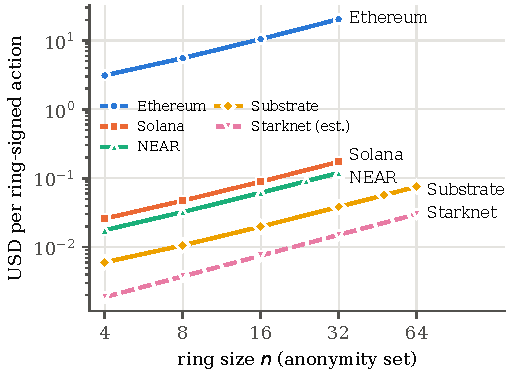
\includegraphics[width=\linewidth]{figures/usd_by_ring.pdf}
\caption{USD per ring-signed action (log--log). Starknet (dashed) is extrapolated linearly from its measured ring-4 cost.}
\label{fig:usd}
\end{subfigure}\hfill
\begin{subfigure}[t]{0.49\linewidth}
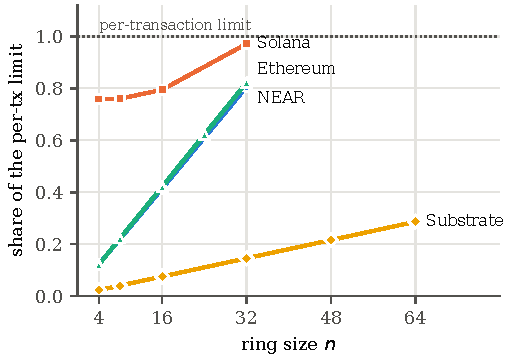
\includegraphics[width=\linewidth]{figures/limit_share.pdf}
\caption{Share of the per-transaction limit used by one submit. For Solana this is the largest single verification unit.}
\label{fig:limit}
\end{subfigure}
\caption{Cost against anonymity-set size. Each series is labelled directly; the values are in Tables~\ref{tab:model} and~\ref{tab:econ}.}
\end{figure}

\begin{table}[t]
\centering\small
\begin{tabular}{@{}llrrrrrr@{}}
\toprule
chain & token & block (s) & 1\,h tempo (blocks) & USD, $n=4$ & $n=32$ & $n=64$ & actions/block \\
\midrule
\tabinput{generated/tab_econ.tex}
\bottomrule
\end{tabular}
\caption{Mainnet economics on \snapdate: USD per ring-signed action by ring size, the number of blocks in the one-hour minimum epoch that public deployments enforce, and how many ring-4 scores one block can carry under the chain's capacity limit. Substrate is priced on Astar, whose fee is linear in ref\_time (327.4\,ASTR per second of weight, times a fee multiplier of 0.1 on that day) plus a length fee; it does not charge for proof\_size. Starknet's capacity is not limited by the actions we measured.}
\label{tab:econ}
\end{table}

\paragraph{Observations.} (1) For every chain we fitted, cost is linear in the anonymity set (Fig.~\ref{fig:usd}). The privacy-cost trade-off is therefore explicit: doubling the anonymity set roughly doubles the fee. (2) Native curve support matters most on Ethereum. With no STARK-curve precompile and an L1 gas price, a ring-4 action costs dollars there, 600 to 1\,900 times more than on Substrate or Starknet. (3) The wasm environments differ mainly in metering and price. NEAR and Substrate execute the \emph{same} verifier source. NEAR charges $\approx7.5$\,Tgas per member against a 300\,Tgas cap. Substrate charges $\approx5.7$\,ms per member against 1.3\,s: each member uses about a sixth as large a share of its limit (0.44\% against 2.5\%). (4) \emph{Settle} is cheap everywhere, because it reads at most 101 histogram entries and verifies no signature.

\section{Reducing cost without giving up privacy}\label{sec:cost}

Table~\ref{tab:econ} prices one action. A subnet pays for an epoch, and in an epoch the contract of Section~\ref{sec:protocol} executes
\[
\underbrace{M\,\mathrm{sub}(n)}_{\text{submit}} + \underbrace{V M\,\mathrm{sig}(n)}_{\text{score}} + \underbrace{M\,\mathrm{set}}_{\text{settle}} + \underbrace{M\,\mathrm{clm}(n)}_{\text{claim}}
\]
with $M$ miners, $V$ validators and ring size $n$, where $\mathrm{sig}(n)=a+bn$ is the fitted model of Table~\ref{tab:model}. The score term grows with the \emph{product} of the two sets, and each of its terms is a full ring verification. At the size of one Bittensor subnet ($M=\scaleM$, $V=\scaleV$, $n=\scalering$, one-hour epochs) it dominates the bill on every chain (first column of Table~\ref{tab:scale}). Cost can be cut in three ways. Some cuts leak nothing, some trade security for cost, and some trade unlinkability for cost. We separate them because the obvious cuts are in the last group.

\paragraph{Free levers.} (i) \emph{Epoch length.} An epoch is the same set of transactions whatever its length, so the cost per day falls as $1/\text{hours}$. Longer epochs reveal nothing new; they only delay payouts. (ii) \emph{Ring size as a privacy floor.} Cost is linear in $n$ (Fig.~\ref{fig:usd}). A deployment should therefore choose the smallest $n$ it accepts as an anonymity set, set $n_{\min}=n$ on chain, and let the client's fixed partition (Section~\ref{sec:intersection}) give every member exactly that set. Members gain nothing by paying for a larger ring, since their linked actions must use the same block anyway. (iii) \emph{Chain.} At equal privacy the same epoch costs \scaleChainSpread{} times more on the most expensive chain (Ethereum L1) than on the cheapest (Starknet) (Table~\ref{tab:scale}). (iv) \emph{Relay batching.} One relayer transaction can carry many members' payloads. That saves only the per-transaction base fee (21\,000 gas against $\approx$2.3\,Mgas on Ethereum, one signature fee on Solana), but it also mixes senders, so it improves privacy.

\paragraph{Cuts that link actions.} The standard compressions all work by merging signatures.
\emph{Batch}: a validator signs its whole score vector once per epoch, as Bittensor's \texttt{set\_weights} does, with one nullifier per (epoch). That replaces $VM$ verifications with $V$. \emph{Lazy}: a miner claims $K$ epochs with one signature. \emph{Proof}: on top of both, every signature is checked off chain and the epoch lands as one validity proof. Each step breaks part of (P5). Batching publishes one validator's scores for every tag, under one nullifier, as a vector. The vector links those scores to each other, and its pattern can fingerprint the validator across epochs, which is exactly the persistent identity the nullifiers were chosen to destroy. A lazy claim links $K$ of a miner's epoch tags, as claiming $K$ times to one address would.

\paragraph{Cuts that keep (P5).} Two changes keep every signature exactly as it is: one tag per miner per epoch, one nullifier per validator per tag.

\emph{Secret committees (sortition).} A validator may score tag $\tg$ only if
\[
\Hs(\nu) < \frac{C}{V}\cdot p, \qquad \nu = \mathrm{id}\big(x\cdot\Hp(\sigma_{e,\tg})\big),
\]
the nullifier it would publish anyway, with $\Hs(\nu)$ read as an integer in $[0,p)$. Only the validator can compute $\nu$, and the ring signature that publishes it also proves the selection, so the contract checks one extra comparison. The committee is unknown until its members act, anyone can verify it, and it reveals nothing beyond the nullifier, so (P5) holds unchanged. A key cannot be ground for a favourable committee, because $\nu$ is fixed by the key and the scope. To stop a coalition from grinding \emph{miner} keys against the coalition's committees before registering them, the scope must include an epoch beacon fixed after the registries freeze for that epoch. A tag then draws about $C$ scores instead of $V$, so the score term becomes $CM\,\mathrm{sig}(n)$.

\emph{Private settlement.} Every submit, score and claim is verified off chain, and one validity proof per epoch states that all signatures verify against the registries, that their images are distinct in their scopes, and that Zuma consensus gives the published results. The images are scoped to the epoch, so their uniqueness can be checked entirely inside the proof; they never need to be stored. On chain remain one proof verification, $M$ tags, $M$ results and $M$ claim records. The prover sees only what is public today: anonymous signatures. It is trusted for liveness, not for soundness. It can omit actions but not forge them, so the direct path of Section~\ref{sec:protocol} stays open as a fallback, and anyone may submit a competing proof that includes more actions. Individual scores need not be published at all, only each tag's $(C_\tg,R_\tg)$. That is \emph{more} private than the baseline, which reveals each score's value. Claims are made once per epoch, each to a fresh recipient, so no tags are linked.

\begin{table}[t]
\centering\small
\begin{tabular}{@{}lrrrrrrr@{}}
\toprule
& & \multicolumn{3}{c}{links actions} & \multicolumn{2}{c}{keeps (P5)} & \\
\cmidrule(lr){3-5}\cmidrule(lr){6-7}
chain & today & batch & +lazy & +proof & committee & +private & saving \\
\midrule
\tabinput{generated/tab_scale.tex}
\bottomrule
\end{tabular}
\caption{USD per day for a Bittensor-sized subnet ($M=\scaleM$ miners, $V=\scaleV$ validators, ring $n=\scalering$, one-hour epochs) at the prices of \snapdate. ``Today'' applies the measured per-action costs. The other columns are modeled (\texttt{src/core/forecast.py}): lazy claims $K=\scaleK$ epochs at once, committees have expected size $C=\scaleC$, a written entry is priced at a quarter of a measured settle, off-chain proving at USD~$10^{-4}$ per million Cairo steps (about $4\,000$ steps per ring member), and the on-chain proof check as a Groth16 wrap (350\,kgas on Ethereum, 300\,kCU on Solana, 30\,Tgas on NEAR, $5\times10^7$ L2 gas for a Garaga verifier on Starknet). $^*$No proof-verifier estimate; priced at 30 ring-16 scores. ``Saving'' is today over +private.}
\label{tab:scale}
\end{table}

\begin{table}[t]
\centering\small
\begin{tabular}{@{}rrrrrrrr@{}}
\toprule
& & \multicolumn{3}{c}{capture} & \multicolumn{3}{c}{starve} \\
\cmidrule(lr){3-5}\cmidrule(lr){6-8}
$V$ & $C$ & $f=0.10$ & $0.25$ & $1/3$ & $0.10$ & $0.25$ & $1/3$ \\
\midrule
\tabinput{generated/tab_capture.tex}
\bottomrule
\end{tabular}
\caption{The security price of committees, per tag. A coalition holds a fraction $f$ of the $V$ validators. Each validator is selected independently with probability $C/V$, and the committee quorum is $\lceil\max(C, n_\tg)/2\rceil$. \emph{Capture}: the coalition reaches the quorum while every honest member drawn votes, so it sets the tag's consensus. \emph{Starve}: fewer than $\lceil C/2\rceil$ honest members are drawn, so a coalition that abstains zeroes the tag. With $C\ge V$ both are $0$ for $f<\tfrac12$ (Proposition~\ref{prop:clip}).}
\label{tab:capture}
\end{table}

\paragraph{The price of committees is security, not privacy.} Zuma's clipping bound (Proposition~\ref{prop:clip}) now holds per committee. We keep the rule $V_\tg=\max(V,n_\tg)$ in committee form, with quorum $k_\tg=\lceil\max(C,n_\tg)/2\rceil$. A coalition with fewer than $C/2$ members can then never reach the quorum. A larger one reaches it on a tag only when the draw favours it (Table~\ref{tab:capture}). With $V=\scaleV$, $C=\scaleC$ and a quarter of the validators colluding, a tag is captured with probability $\capDefault$ and starved with probability $\starveDefault$. With $C=16$ these become $\capSixteen$ and $\starveSixteen$. Starved tags can be re-scored by a second committee drawn in a retry scope; that costs another $C$ scores, but only for starved tags. Committees save the most when $V\gg C$: for $V=\scaleV$ and $C=\scaleC$ they halve the score term, while for $V=256$ they cut it by a factor of eight.

\paragraph{What the numbers say.} Once verification moves off chain, ring size and signature count cost only prover time. At that point linking actions buys almost nothing: on every chain, +private costs the same order per day as +proof, and less on NEAR, Ethereum and Solana, where it also moves claims into the proof (Table~\ref{tab:scale}), and it costs \scaleMinRatio{} to \scaleMaxRatio{} times less than today's contract. The cuts that link actions only pay off when no prover is available. We therefore recommend the second ladder: committees first, because they need only one comparison in the existing contracts, then private settlement. These figures are models of contract changes we have not deployed. The baseline column is the only measured one.

\section{Limitations and threats to validity}\label{sec:limits}

\paragraph{The anonymity set is the ring, and rings are small.} A score from a ring of 4 hides its validator among 4. Rings are canonical and their minimum size is enforced on chain, so a ring cannot be padded, but no contract can create members who do not exist. With a few validators the guarantee is weak, regardless of the cryptography.

\paragraph{Ring intersection: a leak in our earlier ring selection, and the fix.}\label{sec:intersection}
A claim intentionally shares its key image with its submission (P3). In earlier versions, the client sampled a \emph{fresh random} ring for every action whenever the role had more members than the maximum ring. The submission and the claim then show two different rings with the same image. Any observer can intersect them, and the claimant's effective anonymity set falls from $n$ to the overlap: about $n^2/|\mathcal{M}|$ members on average, and one member in the worst case. This is the ring-intersection attack known from Monero~\cite{kumar17,moser18}. It did not affect the evaluation, where every set fit within one ring, but it would affect any deployment whose set exceeds $n_{\max}$. The client now partitions each registry, in registration order, into fixed blocks of $n$ members; the last block borrows from the one before so that every block is full. A member always signs with its own block, so the two linked actions show the same $n$ keys and intersection reveals nothing. A residual leak remains when registrations between a submission and its claim reshuffle the last, partial block. We test the partition rule; enforcing a canonical ring per (scope, member) \emph{on chain} remains open.

\paragraph{Metadata.} The relayer's identity, the time of posting, network addresses and the content of the work can each identify a member. A miner whose work is recognisable is not anonymous to the validators who read it. Relaying through independent relayers and mixing submission times are operational requirements, not features of the protocol.

\paragraph{Collusion and Sybils.} Proposition~\ref{prop:clip} assumes that fewer than half of the snapshot validators collude. Anyone who controls admission to $\mathcal{V}$ can violate that assumption. Sybil resistance is out of scope~\cite{sybil}.

\paragraph{No quantum security.} Unforgeability rests on discrete logarithms and anonymity on DDH in $\G$, and Shor's algorithm~\cite{shor94} breaks both. A quantum adversary can forge signatures and can link key images to keys retroactively. The postquant deployment signs each state transition with ML-DSA~\cite{fips204}. That makes the \emph{history} tamper-evident against such an adversary but does nothing for anonymity. Post-quantum linkable ring signatures from lattices exist~\cite{matrict}, as do hash-based membership proofs from STARKs~\cite{stark}; adopting one is the main open direction.

\paragraph{The cost reductions are modeled.} Committees and private settlement (Section~\ref{sec:cost}) are not deployed. Their costs rest on estimates of a written entry, of proving speed and of each chain's proof-verification cost. Committees weaken the deterministic sub-quorum bound to the probabilistic one of Table~\ref{tab:capture}, and private settlement adds a prover that can delay an epoch, though it cannot forge one.

\paragraph{Validator rewards.} Zuma consensus pays miners only (Section~\ref{sec:zuma}). Validator rewards that preserve nullifier unlinkability are future work.

\paragraph{Threats to validity.} The costs are local measurements. Mainnet costs differ where fee markets add priority fees, or where account abstraction adds validation cost, as on Starknet. Starknet's USD figure is an estimate from Sierra-gas weights, and its by-ring curve is extrapolated from ring 4. Ethereum's figure uses the base fee observed on the snapshot date and moves linearly with it. The proofs in Section~\ref{sec:security} are sketches in the random-oracle model, modelling Poseidon as a random oracle. That is a standard assumption, but not a reduction to Poseidon's concrete security. Finally, all six verifiers are tested against the same signer. A bug common to the signer and every verifier would not be caught by cross-chain agreement. It would have to survive the independent Cairo, Solidity and sBPF implementations as well as the shared Rust sources.

\section{Conclusion}

The rules of an incentive subnet can be enforced without the identities that currently enforce them. A single linkable ring signature, used in three carefully chosen scopes, gives one submission per miner per epoch, one score per validator per submission, and a claim only the earner can make. Zuma consensus keeps Yuma's majority clipping with anonymous, equally weighted validators. The cost is linear in the anonymity set and fits comfortably within transaction limits on Starknet and Substrate. On NEAR and Solana it is bounded at 32 members, and on Ethereum L1 it is expensive. At scale the cost is driven by miners times validators. It can be cut by orders of magnitude without linking any action: secret committees drawn from the nullifiers, then one validity proof per epoch. The cheaper-looking batched weights and lazy claims give up unlinkability for savings that vanish once a prover exists. The limits are equally concrete: small sets give small anonymity, metadata can betray members, the construction is not post-quantum, and validator rewards remain open.

\appendix
\section{Reproducing the results}\label{app:repro}
\begin{small}
\begin{verbatim}
python3 -m pytest                          # offline: codecs, adapters, Zuma, ring rule
ZTAO_NATIVE=1 python3 -m pytest -m native   # snforge, cargo, forge suites
ZTAO_LIVE=1   python3 -m pytest -m live     # one full epoch per local chain
m ztao/simulate chain=substrate         # epoch on substrate-contracts-node :51507
m ztao/gas_sweep chain=substrate sizes=4,8,16,32,48,64
m ztao/forecast chain=near miners=16,256 validators=4,64   # both ladders
m ztao/experiment chain=near strategy=private
python3 paper/collect.py && python3 paper/figures.py && ./paper/build.sh
\end{verbatim}
\end{small}

\bibliographystyle{plainnat}
\bibliography{refs}

\end{document}
